\documentclass[]{article}
\usepackage{lmodern}
\usepackage{amssymb,amsmath}
\usepackage{ifxetex,ifluatex}
\usepackage{fixltx2e} % provides \textsubscript
\ifnum 0\ifxetex 1\fi\ifluatex 1\fi=0 % if pdftex
  \usepackage[T1]{fontenc}
  \usepackage[utf8]{inputenc}
\else % if luatex or xelatex
  \ifxetex
    \usepackage{mathspec}
  \else
    \usepackage{fontspec}
  \fi
  \defaultfontfeatures{Ligatures=TeX,Scale=MatchLowercase}
\fi
% use upquote if available, for straight quotes in verbatim environments
\IfFileExists{upquote.sty}{\usepackage{upquote}}{}
% use microtype if available
\IfFileExists{microtype.sty}{%
\usepackage{microtype}
\UseMicrotypeSet[protrusion]{basicmath} % disable protrusion for tt fonts
}{}
\usepackage[margin=1in]{geometry}
\usepackage{hyperref}
\hypersetup{unicode=true,
            pdftitle={Report: Hybrid vigor in response to Eimeria in the HMHZ},
            pdfauthor={Alice},
            pdfborder={0 0 0},
            breaklinks=true}
\urlstyle{same}  % don't use monospace font for urls
\usepackage{color}
\usepackage{fancyvrb}
\newcommand{\VerbBar}{|}
\newcommand{\VERB}{\Verb[commandchars=\\\{\}]}
\DefineVerbatimEnvironment{Highlighting}{Verbatim}{commandchars=\\\{\}}
% Add ',fontsize=\small' for more characters per line
\usepackage{framed}
\definecolor{shadecolor}{RGB}{248,248,248}
\newenvironment{Shaded}{\begin{snugshade}}{\end{snugshade}}
\newcommand{\KeywordTok}[1]{\textcolor[rgb]{0.13,0.29,0.53}{\textbf{#1}}}
\newcommand{\DataTypeTok}[1]{\textcolor[rgb]{0.13,0.29,0.53}{#1}}
\newcommand{\DecValTok}[1]{\textcolor[rgb]{0.00,0.00,0.81}{#1}}
\newcommand{\BaseNTok}[1]{\textcolor[rgb]{0.00,0.00,0.81}{#1}}
\newcommand{\FloatTok}[1]{\textcolor[rgb]{0.00,0.00,0.81}{#1}}
\newcommand{\ConstantTok}[1]{\textcolor[rgb]{0.00,0.00,0.00}{#1}}
\newcommand{\CharTok}[1]{\textcolor[rgb]{0.31,0.60,0.02}{#1}}
\newcommand{\SpecialCharTok}[1]{\textcolor[rgb]{0.00,0.00,0.00}{#1}}
\newcommand{\StringTok}[1]{\textcolor[rgb]{0.31,0.60,0.02}{#1}}
\newcommand{\VerbatimStringTok}[1]{\textcolor[rgb]{0.31,0.60,0.02}{#1}}
\newcommand{\SpecialStringTok}[1]{\textcolor[rgb]{0.31,0.60,0.02}{#1}}
\newcommand{\ImportTok}[1]{#1}
\newcommand{\CommentTok}[1]{\textcolor[rgb]{0.56,0.35,0.01}{\textit{#1}}}
\newcommand{\DocumentationTok}[1]{\textcolor[rgb]{0.56,0.35,0.01}{\textbf{\textit{#1}}}}
\newcommand{\AnnotationTok}[1]{\textcolor[rgb]{0.56,0.35,0.01}{\textbf{\textit{#1}}}}
\newcommand{\CommentVarTok}[1]{\textcolor[rgb]{0.56,0.35,0.01}{\textbf{\textit{#1}}}}
\newcommand{\OtherTok}[1]{\textcolor[rgb]{0.56,0.35,0.01}{#1}}
\newcommand{\FunctionTok}[1]{\textcolor[rgb]{0.00,0.00,0.00}{#1}}
\newcommand{\VariableTok}[1]{\textcolor[rgb]{0.00,0.00,0.00}{#1}}
\newcommand{\ControlFlowTok}[1]{\textcolor[rgb]{0.13,0.29,0.53}{\textbf{#1}}}
\newcommand{\OperatorTok}[1]{\textcolor[rgb]{0.81,0.36,0.00}{\textbf{#1}}}
\newcommand{\BuiltInTok}[1]{#1}
\newcommand{\ExtensionTok}[1]{#1}
\newcommand{\PreprocessorTok}[1]{\textcolor[rgb]{0.56,0.35,0.01}{\textit{#1}}}
\newcommand{\AttributeTok}[1]{\textcolor[rgb]{0.77,0.63,0.00}{#1}}
\newcommand{\RegionMarkerTok}[1]{#1}
\newcommand{\InformationTok}[1]{\textcolor[rgb]{0.56,0.35,0.01}{\textbf{\textit{#1}}}}
\newcommand{\WarningTok}[1]{\textcolor[rgb]{0.56,0.35,0.01}{\textbf{\textit{#1}}}}
\newcommand{\AlertTok}[1]{\textcolor[rgb]{0.94,0.16,0.16}{#1}}
\newcommand{\ErrorTok}[1]{\textcolor[rgb]{0.64,0.00,0.00}{\textbf{#1}}}
\newcommand{\NormalTok}[1]{#1}
\usepackage{longtable,booktabs}
\usepackage{graphicx,grffile}
\makeatletter
\def\maxwidth{\ifdim\Gin@nat@width>\linewidth\linewidth\else\Gin@nat@width\fi}
\def\maxheight{\ifdim\Gin@nat@height>\textheight\textheight\else\Gin@nat@height\fi}
\makeatother
% Scale images if necessary, so that they will not overflow the page
% margins by default, and it is still possible to overwrite the defaults
% using explicit options in \includegraphics[width, height, ...]{}
\setkeys{Gin}{width=\maxwidth,height=\maxheight,keepaspectratio}
\IfFileExists{parskip.sty}{%
\usepackage{parskip}
}{% else
\setlength{\parindent}{0pt}
\setlength{\parskip}{6pt plus 2pt minus 1pt}
}
\setlength{\emergencystretch}{3em}  % prevent overfull lines
\providecommand{\tightlist}{%
  \setlength{\itemsep}{0pt}\setlength{\parskip}{0pt}}
\setcounter{secnumdepth}{0}
% Redefines (sub)paragraphs to behave more like sections
\ifx\paragraph\undefined\else
\let\oldparagraph\paragraph
\renewcommand{\paragraph}[1]{\oldparagraph{#1}\mbox{}}
\fi
\ifx\subparagraph\undefined\else
\let\oldsubparagraph\subparagraph
\renewcommand{\subparagraph}[1]{\oldsubparagraph{#1}\mbox{}}
\fi

%%% Use protect on footnotes to avoid problems with footnotes in titles
\let\rmarkdownfootnote\footnote%
\def\footnote{\protect\rmarkdownfootnote}

%%% Change title format to be more compact
\usepackage{titling}

% Create subtitle command for use in maketitle
\newcommand{\subtitle}[1]{
  \posttitle{
    \begin{center}\large#1\end{center}
    }
}

\setlength{\droptitle}{-2em}

  \title{Report: Hybrid vigor in response to Eimeria in the HMHZ}
    \pretitle{\vspace{\droptitle}\centering\huge}
  \posttitle{\par}
    \author{Alice}
    \preauthor{\centering\large\emph}
  \postauthor{\par}
      \predate{\centering\large\emph}
  \postdate{\par}
    \date{15 October 2018}

\usepackage{float} 
\let\origfigure\figure 
\let\endorigfigure\endfigure 
\renewenvironment{figure}[1][2] { 
    \expandafter\origfigure\expandafter[H] 
} { 
    \endorigfigure 
}

\begin{document}
\maketitle

{
\setcounter{tocdepth}{4}
\tableofcontents
}
\section{Eimeria detection oocysts
flotation}\label{eimeria-detection-oocysts-flotation}

\subsection{Improving Eimeria oocysts
detection}\label{improving-eimeria-oocysts-detection}

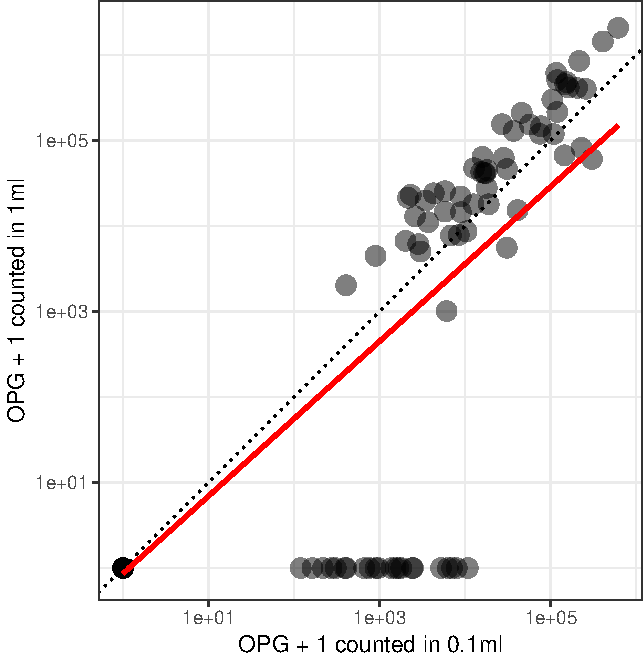
\includegraphics{Data_Analysis_Alice_files/figure-latex/oocystsDetec-1.pdf}

22 new samples were detected while diluting by 0.1mL PBS instead of 1mL
before counting in Neubauer chamber.

Adjusted R-squared = 0.81 represents the amount of variation in y
explained by x.

\subsection{OPG that we keep}\label{opg-that-we-keep}

Number of Mus musculus caught with OPG values: 484

\begin{verbatim}
## `geom_smooth()` using method = 'loess' and formula 'y ~ x'
\end{verbatim}

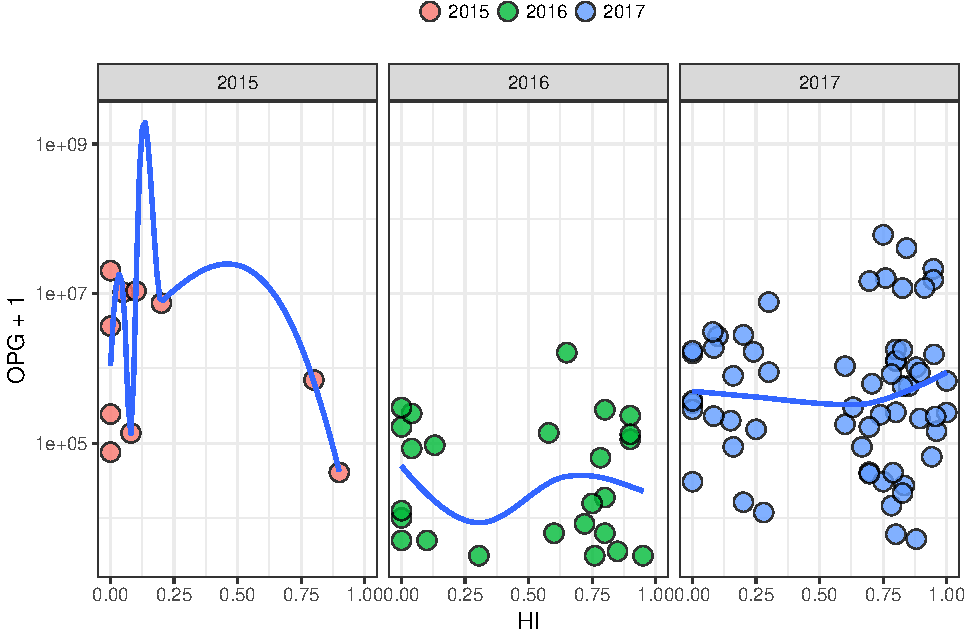
\includegraphics{Data_Analysis_Alice_files/figure-latex/oocystssmooth-1.pdf}

\section{Eimeria detection PCR}\label{eimeria-detection-pcr}

PCR positive = one of the 3 other markers than AP5 sequenced (Ap5 was
used for detection only, the other markers for confirmation)

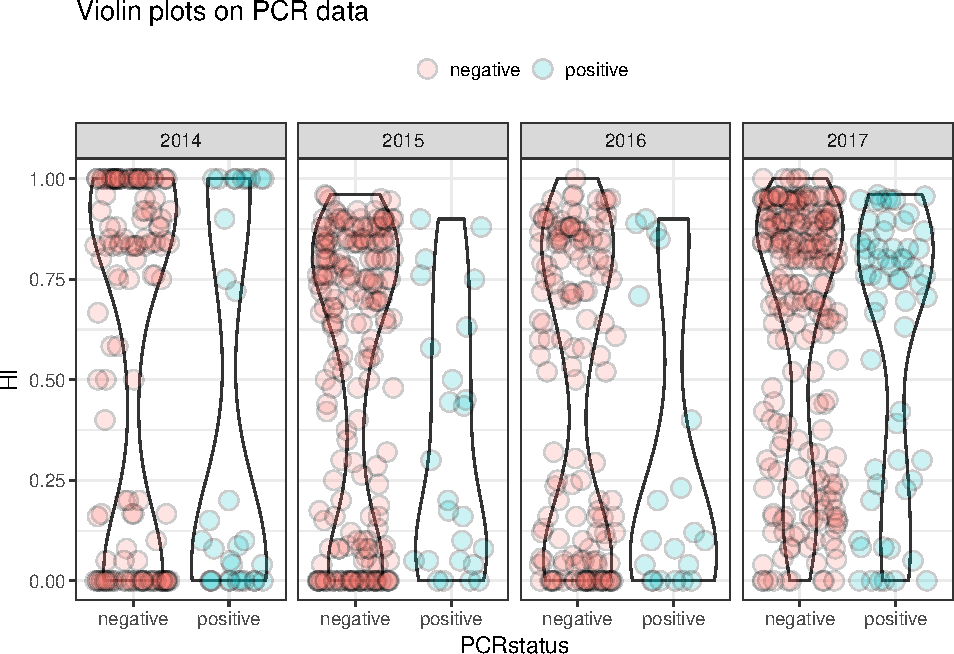
\includegraphics{Data_Analysis_Alice_files/figure-latex/pcr-1.pdf}

PCR positive = one of the 3 markers 18S, COI or ORF470) gave a sequence.
Number of Mus musculus caught with PCR performed: 1165

\section{Eimeria detection qPCR}\label{eimeria-detection-qpcr}

We keep only the values for mice having been tested for BOTH ileum and
cecum!

\begin{verbatim}
## `geom_smooth()` using method = 'loess' and formula 'y ~ x'
\end{verbatim}

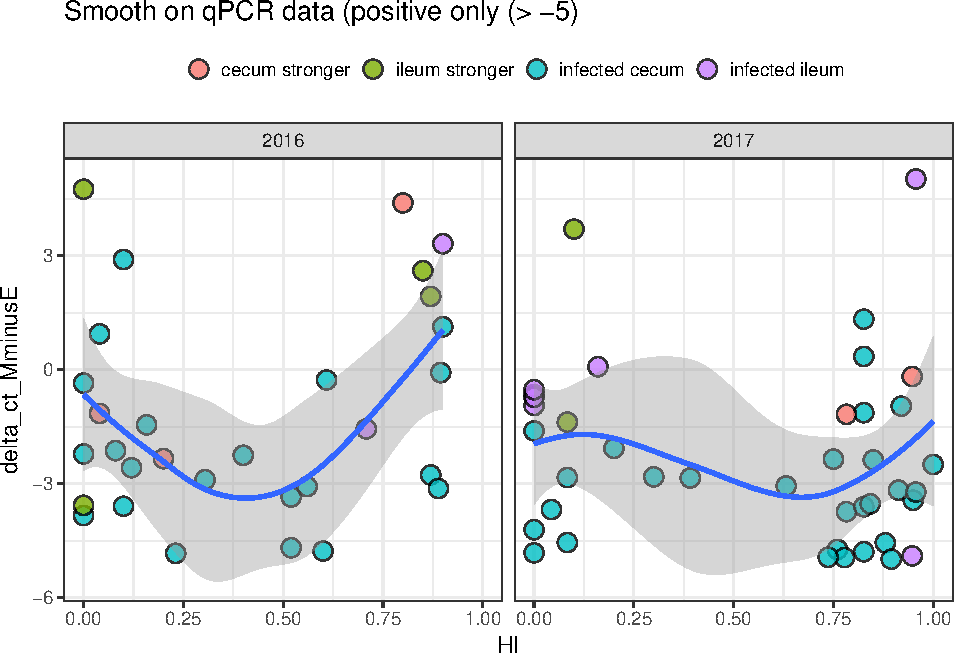
\includegraphics{Data_Analysis_Alice_files/figure-latex/qpcr-1.pdf}

\begin{verbatim}
## Warning: Removed 107 rows containing missing values (geom_point).
\end{verbatim}

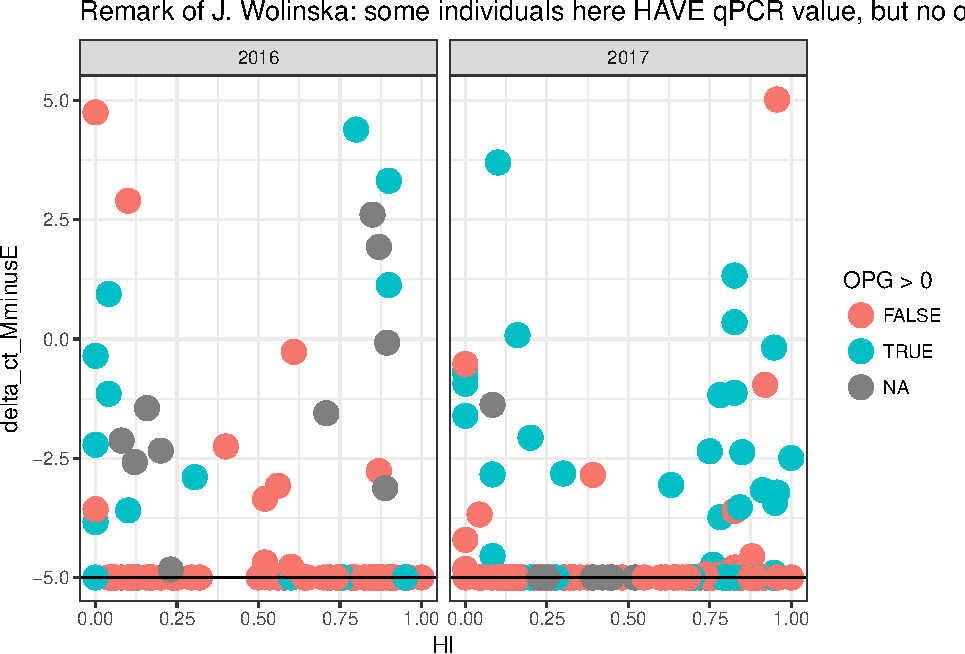
\includegraphics{Data_Analysis_Alice_files/figure-latex/qpcr-2.pdf}

\section{General stats on sampling}\label{general-stats-on-sampling}

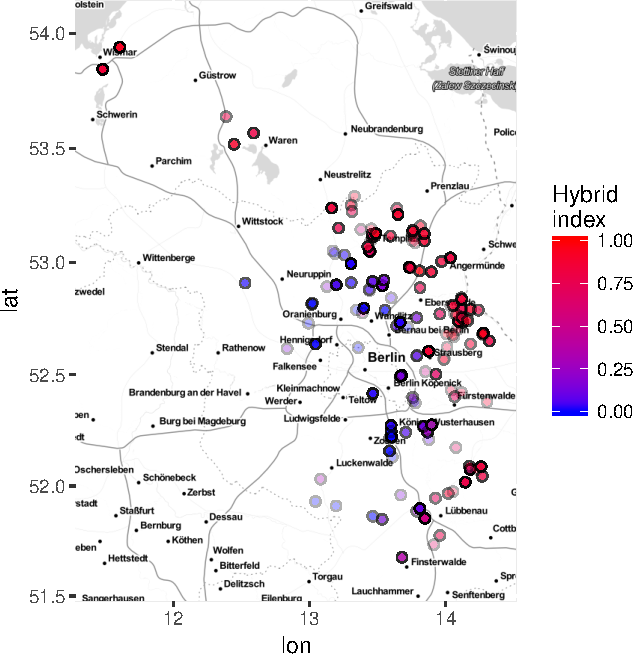
\includegraphics{Data_Analysis_Alice_files/figure-latex/generalstats-1.pdf}

\begin{itemize}
\tightlist
\item
  Some information regarding latitude and longitude are missing for the
  following mice:
\end{itemize}

AA\_0080c, AA\_0080i, AA\_0100c, SK\_2903, SK\_2904, SK\_2958, SK\_2959,
SK\_2960, SK\_2961, SK\_3174, SK\_3333, SK\_3417, SK\_3461, SK\_3462,
SK\_3469, SK\_3470, SK\_3471

\begin{itemize}
\tightlist
\item
  We still miss info (HI) on the following mice (ask Jarda):
\end{itemize}

AA\_0080c, AA\_0080i, AA\_0100c, AA\_0411, AA\_0412, AA\_0420, AA\_0464,
SK\_2668, SK\_2669, SK\_2671, SK\_2674, SK\_2675, SK\_2676, SK\_2677,
SK\_2678, SK\_2681, SK\_2682, SK\_2684, SK\_2685, SK\_2687, SK\_2688,
SK\_2690, SK\_2692, SK\_2693, SK\_2695, SK\_2696, SK\_2699, SK\_2700,
SK\_2701, SK\_2702, SK\_2703, SK\_2704, SK\_2705, SK\_2710, SK\_2713,
SK\_2715, SK\_2724, SK\_2727, SK\_2729, SK\_2733, SK\_2734, SK\_2736,
SK\_2737, SK\_2738, SK\_2739, SK\_2745, SK\_2750, SK\_2751, SK\_2752,
SK\_2754, SK\_2755, SK\_2756, SK\_2758, SK\_2759, SK\_2760, SK\_2761,
SK\_2775, SK\_2778, SK\_2780, SK\_2782, SK\_2789, SK\_2792, SK\_2793,
SK\_2794, SK\_2795, SK\_2798, SK\_2799, SK\_2800, SK\_2801, SK\_2802,
SK\_2803, SK\_2804, SK\_2805, SK\_2851, SK\_2852, SK\_2853, SK\_2854,
SK\_2855, SK\_2856, SK\_2857, SK\_2858, SK\_2859, SK\_2860, SK\_2861,
SK\_2862, SK\_2863, SK\_2864, SK\_2865, SK\_2866, SK\_2868, SK\_2869,
SK\_2870, SK\_2871, SK\_2873, SK\_2874, SK\_2875, SK\_2876, SK\_2877,
SK\_2878, SK\_2879, SK\_2880, SK\_2881, SK\_2884, SK\_2885, SK\_2886,
SK\_2887, SK\_2888, SK\_2889, SK\_2958, SK\_2959, SK\_2960, SK\_2961,
SK\_3174, SK\_3333, SK\_3417, SK\_3461, SK\_3462, SK\_3469, SK\_3470,
SK\_3471

\section{General informations on
HMHZ}\label{general-informations-on-hmhz}

\begin{itemize}
\item
  1339 mice were captured over three years, from 285 farms
\item
  On average, NA mice were caught per farm (95\% CI NA)
\item
  \textbf{Hybrid indexes} were calculated as ratio of M.m.d/M.m.m
  alleles (between 1 and 14, on average 12 loci)
\end{itemize}

\begin{figure}
\centering
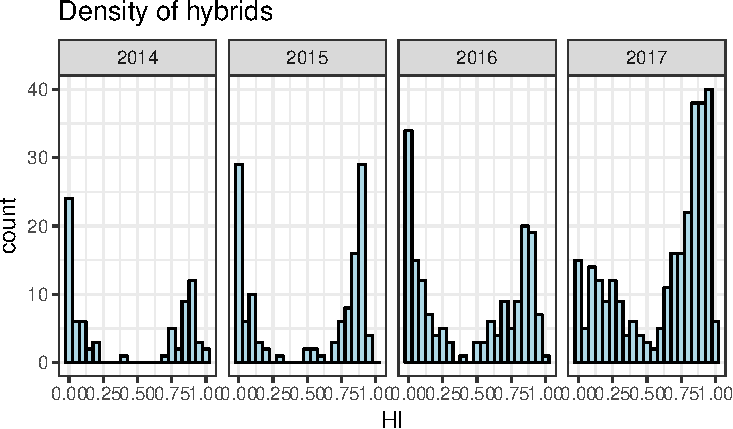
\includegraphics{Data_Analysis_Alice_files/figure-latex/plotDensHI-1.pdf}
\caption{\label{fig:plot1}Number of animals caught along the hybrid
index}
\end{figure}

\section{Prevalence of our 3 different
methods}\label{prevalence-of-our-3-different-methods}

\subsection{Prevalence tables}\label{prevalence-tables}

\begin{longtable}[]{@{}lrrrrrr@{}}
\caption{Prevalence of Eimeria per year, based on oocyst
flotation}\tabularnewline
\toprule
& 2010 & 2011 & 2014 & 2015 & 2016 & 2017\tabularnewline
\midrule
\endfirsthead
\toprule
& 2010 & 2011 & 2014 & 2015 & 2016 & 2017\tabularnewline
\midrule
\endhead
FALSE & 0 & 0 & 0 & 92.0 & 126.00 & 165.00\tabularnewline
TRUE & 0 & 0 & 0 & 10.0 & 25.00 & 65.00\tabularnewline
total & 0 & 0 & 0 & 102.0 & 151.00 & 230.00\tabularnewline
prevalence(\%) & NaN & NaN & NaN & 9.8 & 16.56 & 28.26\tabularnewline
\bottomrule
\end{longtable}

\begin{longtable}[]{@{}lrrrrrr@{}}
\caption{Prevalence of Eimeria per year, based on PCR detection. A mouse
was considered infected by Eimeria if one of the 3 markers (COI, 18S or
ORF470) gave a sequence}\tabularnewline
\toprule
& 2010 & 2011 & 2014 & 2015 & 2016 & 2017\tabularnewline
\midrule
\endfirsthead
\toprule
& 2010 & 2011 & 2014 & 2015 & 2016 & 2017\tabularnewline
\midrule
\endhead
FALSE & 0 & 0 & 241.00 & 417.00 & 149.00 & 207.00\tabularnewline
TRUE & 0 & 0 & 40.00 & 27.00 & 21.00 & 62.00\tabularnewline
total & 0 & 0 & 281.00 & 444.00 & 170.00 & 269.00\tabularnewline
prevalence(\%) & NaN & NaN & 14.23 & 6.08 & 12.35 & 23.05\tabularnewline
\bottomrule
\end{longtable}

\begin{longtable}[]{@{}lrrrrrr@{}}
\caption{Prevalence of Eimeria per year, based on qPCR in
cecum}\tabularnewline
\toprule
& 2010 & 2011 & 2014 & 2015 & 2016 & 2017\tabularnewline
\midrule
\endfirsthead
\toprule
& 2010 & 2011 & 2014 & 2015 & 2016 & 2017\tabularnewline
\midrule
\endhead
FALSE & 0 & 0 & 0 & 0 & 136.00 & 187\tabularnewline
TRUE & 0 & 0 & 0 & 0 & 29.00 & 33\tabularnewline
total & 0 & 0 & 0 & 0 & 165.00 & 220\tabularnewline
prevalence(\%) & NaN & NaN & NaN & NaN & 17.58 & 15\tabularnewline
\bottomrule
\end{longtable}

\begin{longtable}[]{@{}lrrrrrr@{}}
\caption{Prevalence of Eimeria per year, based on all detections
methods. A mouse was considered infected by Eimeria if one of the 3
markers (COI, 18S or ORF470) gave a sequence, OR if it had a positive
count of oocysts in its feces, OR if it was qPCR positive in cecum
tissue}\tabularnewline
\toprule
& 2010 & 2011 & 2014 & 2015 & 2016 & 2017\tabularnewline
\midrule
\endfirsthead
\toprule
& 2010 & 2011 & 2014 & 2015 & 2016 & 2017\tabularnewline
\midrule
\endhead
negative & 49 & 55 & 243.00 & 428.00 & 123.00 & 227.00\tabularnewline
positive & 0 & 0 & 40.00 & 32.00 & 47.00 & 93.00\tabularnewline
total & 49 & 55 & 283.00 & 460.00 & 170.00 & 320.00\tabularnewline
prevalence(\%) & 0 & 0 & 14.13 & 6.96 & 27.65 & 29.06\tabularnewline
\bottomrule
\end{longtable}

\subsection{OPG-PCR}\label{opg-pcr}

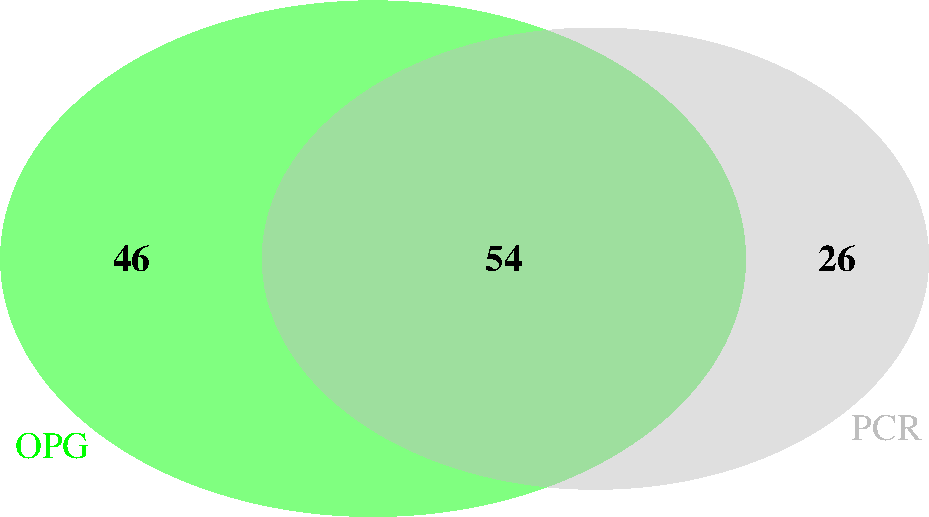
\includegraphics{Data_Analysis_Alice_files/figure-latex/opgpcr-1.pdf}

\begin{verbatim}
## (polygon[GRID.polygon.829], polygon[GRID.polygon.830], polygon[GRID.polygon.831], polygon[GRID.polygon.832], text[GRID.text.833], text[GRID.text.834], text[GRID.text.835], text[GRID.text.836], text[GRID.text.837])
\end{verbatim}

\subsection{OPG-qPCR}\label{opg-qpcr}

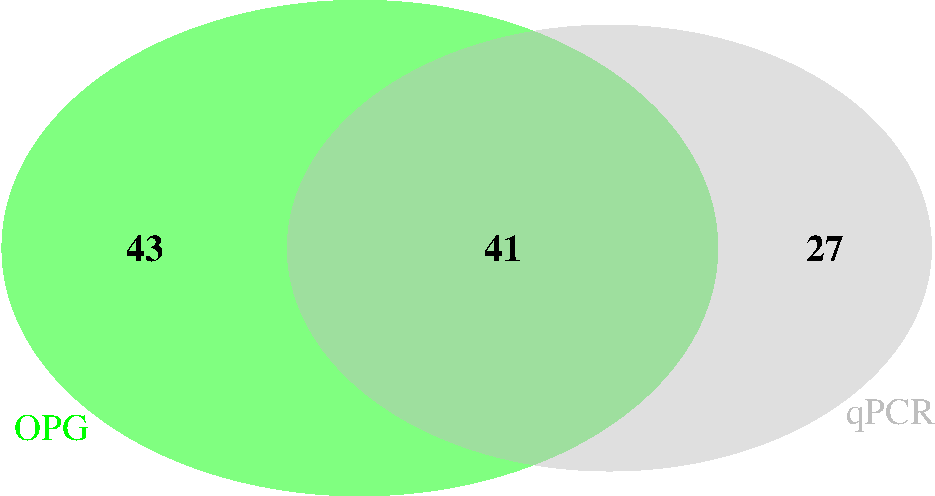
\includegraphics{Data_Analysis_Alice_files/figure-latex/opgpcrVenn-1.pdf}

\begin{verbatim}
## (polygon[GRID.polygon.838], polygon[GRID.polygon.839], polygon[GRID.polygon.840], polygon[GRID.polygon.841], text[GRID.text.842], text[GRID.text.843], text[GRID.text.844], text[GRID.text.845], text[GRID.text.846])
\end{verbatim}

\subsection{OPG-qPCR-PCR}\label{opg-qpcr-pcr}

\section{Testing hybrid vigor along
HMHZ}\label{testing-hybrid-vigor-along-hmhz}

\begin{Shaded}
\begin{Highlighting}[]
\KeywordTok{ggplot}\NormalTok{(miceTable, }\KeywordTok{aes}\NormalTok{(}\DataTypeTok{x =}\NormalTok{ eimeriaSpecies, }\DataTypeTok{y =}\NormalTok{ OPG }\OperatorTok{+}\DecValTok{1}\NormalTok{)) }\OperatorTok{+}
\StringTok{  }\KeywordTok{geom_violin}\NormalTok{() }\OperatorTok{+}
\StringTok{  }\KeywordTok{geom_jitter}\NormalTok{(}\DataTypeTok{width =}\NormalTok{ .}\DecValTok{1}\NormalTok{, }\DataTypeTok{pch =} \DecValTok{21}\NormalTok{, }\DataTypeTok{size =} \DecValTok{2}\NormalTok{) }\OperatorTok{+}
\StringTok{  }\KeywordTok{scale_y_log10}\NormalTok{() }\OperatorTok{+}
\StringTok{  }\KeywordTok{theme_classic}\NormalTok{() }\OperatorTok{+}
\StringTok{  }\KeywordTok{theme}\NormalTok{(}\DataTypeTok{axis.text.x =} \KeywordTok{element_text}\NormalTok{(}\DataTypeTok{angle =} \DecValTok{45}\NormalTok{, }\DataTypeTok{hjust =} \DecValTok{1}\NormalTok{)) }
\end{Highlighting}
\end{Shaded}

\begin{verbatim}
## Warning: Removed 855 rows containing non-finite values (stat_ydensity).
\end{verbatim}

\begin{verbatim}
## Warning: Removed 855 rows containing missing values (geom_point).
\end{verbatim}

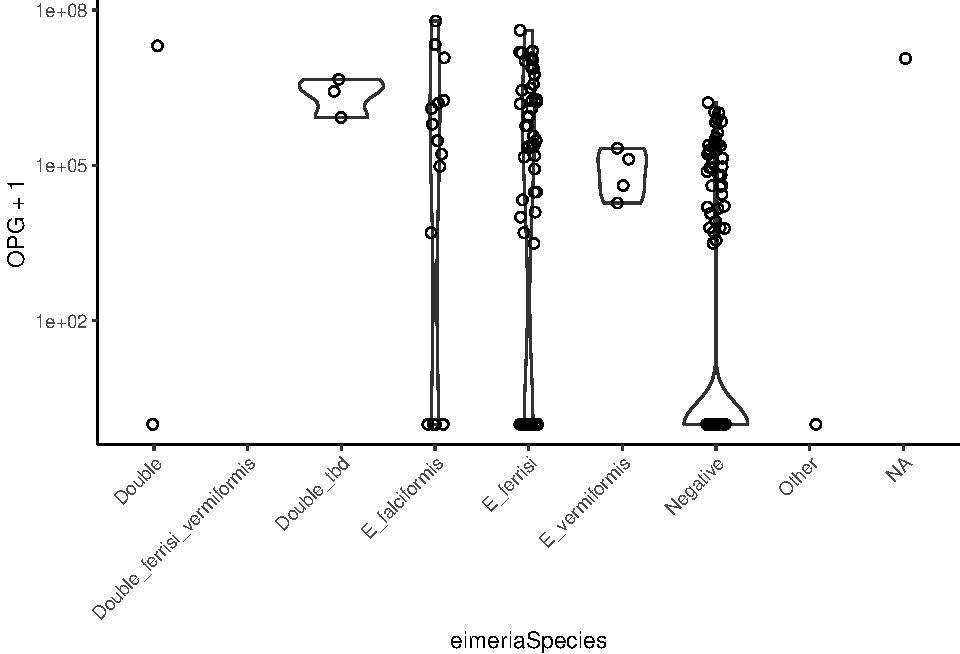
\includegraphics{Data_Analysis_Alice_files/figure-latex/unnamed-chunk-1-1.pdf}

\begin{Shaded}
\begin{Highlighting}[]
\NormalTok{ferrisiDFflot <-}\StringTok{ }\NormalTok{miceTable[}\OperatorTok{!}\KeywordTok{is.na}\NormalTok{(miceTable}\OperatorTok{$}\NormalTok{OPG) }\OperatorTok{&}
\StringTok{                         }\NormalTok{miceTable}\OperatorTok{$}\NormalTok{OPG }\OperatorTok{>}\StringTok{ }\DecValTok{0} \OperatorTok{&}
\StringTok{                         }\OperatorTok{!}\KeywordTok{is.na}\NormalTok{(miceTable}\OperatorTok{$}\NormalTok{eimeriaSpecies) }\OperatorTok{&}
\StringTok{                         }\NormalTok{miceTable}\OperatorTok{$}\NormalTok{eimeriaSpecies }\OperatorTok{==}\StringTok{ "E_ferrisi"}\NormalTok{,]}

\KeywordTok{ggplot}\NormalTok{(ferrisiDFflot, }\KeywordTok{aes}\NormalTok{(}\DataTypeTok{x =}\NormalTok{ HI, }\DataTypeTok{y =}\NormalTok{ OPG)) }\OperatorTok{+}
\StringTok{  }\KeywordTok{geom_point}\NormalTok{() }\OperatorTok{+}
\StringTok{  }\KeywordTok{scale_y_log10}\NormalTok{() }\OperatorTok{+}
\StringTok{  }\KeywordTok{geom_smooth}\NormalTok{()}
\end{Highlighting}
\end{Shaded}

\begin{verbatim}
## `geom_smooth()` using method = 'loess' and formula 'y ~ x'
\end{verbatim}

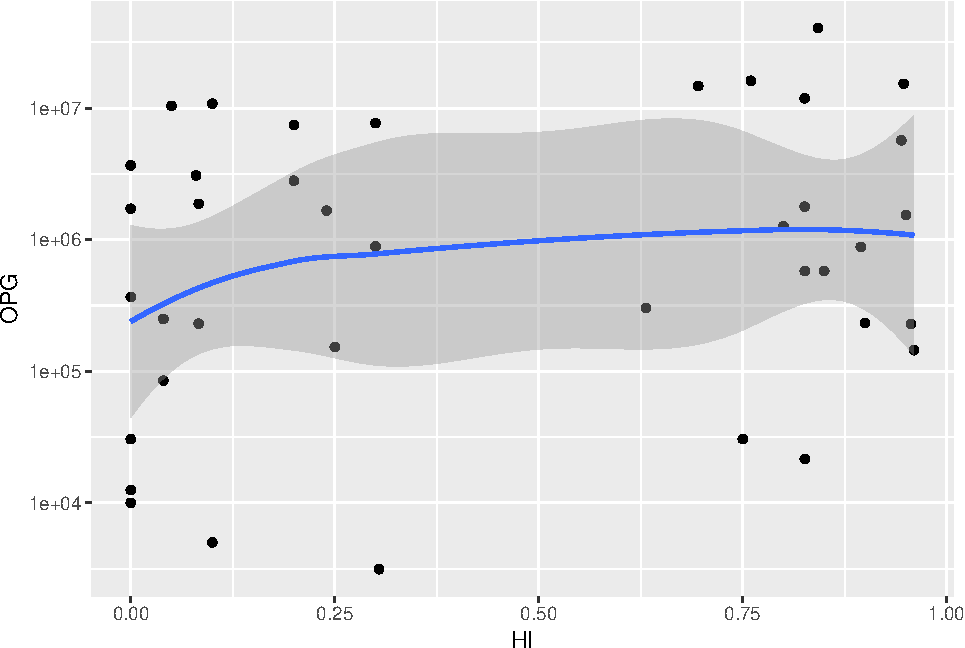
\includegraphics{Data_Analysis_Alice_files/figure-latex/unnamed-chunk-1-2.pdf}

\begin{Shaded}
\begin{Highlighting}[]
\NormalTok{## qPCR by OPG}
\NormalTok{ferrisiDFflot_n_qpcr <-}\StringTok{ }\NormalTok{miceTable[}\OperatorTok{!}\KeywordTok{is.na}\NormalTok{(miceTable}\OperatorTok{$}\NormalTok{OPG) }\OperatorTok{&}
\StringTok{                                    }\NormalTok{miceTable}\OperatorTok{$}\NormalTok{OPG }\OperatorTok{>}\StringTok{ }\DecValTok{0} \OperatorTok{&}
\StringTok{                                    }\OperatorTok{!}\KeywordTok{is.na}\NormalTok{(miceTable}\OperatorTok{$}\NormalTok{delta_ct_cewe_MminusE) }\OperatorTok{&}
\StringTok{                                    }\NormalTok{miceTable}\OperatorTok{$}\NormalTok{delta_ct_cewe_MminusE }\OperatorTok{>}\StringTok{ }\OperatorTok{-}\DecValTok{5} \OperatorTok{&}
\StringTok{                                    }\OperatorTok{!}\KeywordTok{is.na}\NormalTok{(miceTable}\OperatorTok{$}\NormalTok{eimeriaSpecies) }\OperatorTok{&}
\StringTok{                                    }\NormalTok{miceTable}\OperatorTok{$}\NormalTok{eimeriaSpecies }\OperatorTok{==}\StringTok{ "E_ferrisi"}\NormalTok{,]}
  
\KeywordTok{ggplot}\NormalTok{(ferrisiDFflot_n_qpcr, }\KeywordTok{aes}\NormalTok{(}\DataTypeTok{x =}\NormalTok{ delta_ct_cewe_MminusE, }\DataTypeTok{y =}\NormalTok{ OPG)) }\OperatorTok{+}
\StringTok{  }\KeywordTok{geom_point}\NormalTok{() }\OperatorTok{+}
\StringTok{  }\KeywordTok{scale_y_log10}\NormalTok{() }\OperatorTok{+}
\StringTok{  }\KeywordTok{geom_smooth}\NormalTok{(}\DataTypeTok{method =} \StringTok{"lm"}\NormalTok{) }\OperatorTok{+}
\StringTok{  }\KeywordTok{theme_classic}\NormalTok{()}
\end{Highlighting}
\end{Shaded}

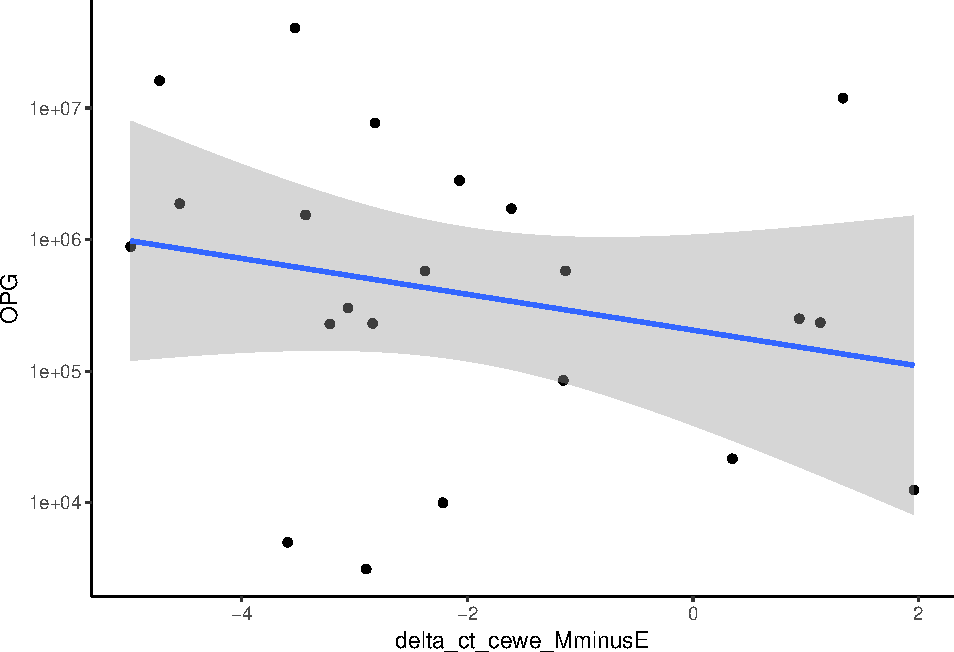
\includegraphics{Data_Analysis_Alice_files/figure-latex/unnamed-chunk-1-3.pdf}

\begin{Shaded}
\begin{Highlighting}[]
\NormalTok{## BCI vs OPG}
\KeywordTok{ggplot}\NormalTok{(ferrisiDFflot, }\KeywordTok{aes}\NormalTok{(}\DataTypeTok{x =}\NormalTok{ BCI, }\DataTypeTok{y =}\NormalTok{ OPG)) }\OperatorTok{+}
\StringTok{  }\KeywordTok{geom_point}\NormalTok{() }\OperatorTok{+}
\StringTok{  }\KeywordTok{scale_y_log10}\NormalTok{() }\OperatorTok{+}
\StringTok{  }\KeywordTok{geom_smooth}\NormalTok{(}\DataTypeTok{method =} \StringTok{"lm"}\NormalTok{) }\OperatorTok{+}
\StringTok{  }\KeywordTok{theme_classic}\NormalTok{()}
\end{Highlighting}
\end{Shaded}

\begin{verbatim}
## Warning: Removed 1 rows containing non-finite values (stat_smooth).
\end{verbatim}

\begin{verbatim}
## Warning: Removed 1 rows containing missing values (geom_point).
\end{verbatim}

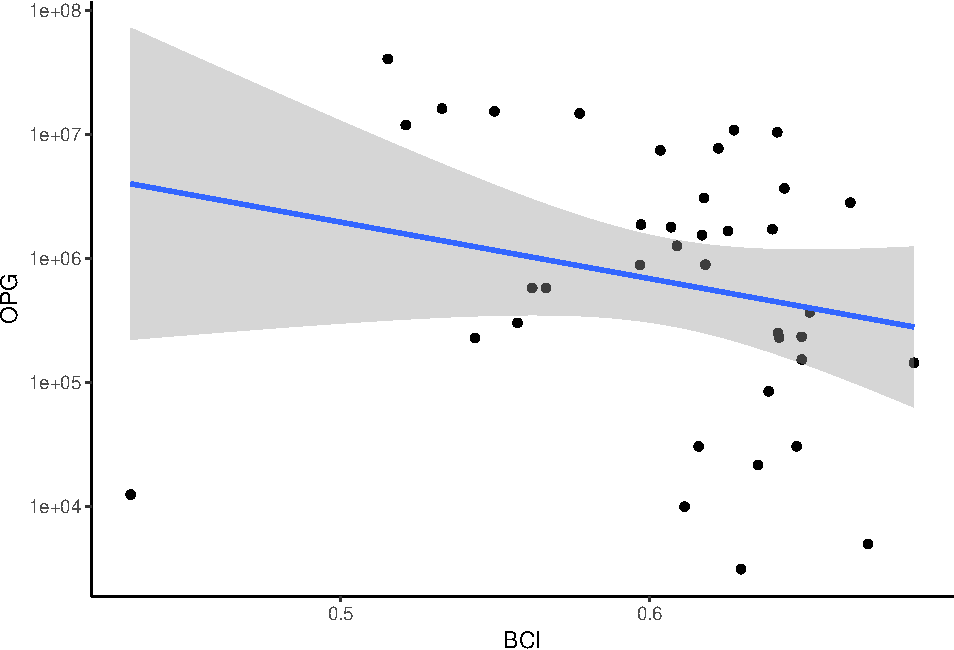
\includegraphics{Data_Analysis_Alice_files/figure-latex/unnamed-chunk-1-4.pdf}

\begin{Shaded}
\begin{Highlighting}[]
\KeywordTok{summary}\NormalTok{(}\KeywordTok{lm}\NormalTok{(ferrisiDFflot}\OperatorTok{$}\NormalTok{BCI }\OperatorTok{~}\StringTok{ }\NormalTok{ferrisiDFflot}\OperatorTok{$}\NormalTok{OPG))}
\end{Highlighting}
\end{Shaded}

\begin{verbatim}
## 
## Call:
## lm(formula = ferrisiDFflot$BCI ~ ferrisiDFflot$OPG)
## 
## Residuals:
##       Min        1Q    Median        3Q       Max 
## -0.186174 -0.013713  0.008491  0.028530  0.067600 
## 
## Coefficients:
##                     Estimate Std. Error t value Pr(>|t|)    
## (Intercept)        6.183e-01  8.720e-03  70.908  < 2e-16 ***
## ferrisiDFflot$OPG -2.764e-09  9.995e-10  -2.765  0.00891 ** 
## ---
## Signif. codes:  0 '***' 0.001 '**' 0.01 '*' 0.05 '.' 0.1 ' ' 1
## 
## Residual standard error: 0.04712 on 36 degrees of freedom
##   (1 observation deleted due to missingness)
## Multiple R-squared:  0.1752, Adjusted R-squared:  0.1523 
## F-statistic: 7.648 on 1 and 36 DF,  p-value: 0.00891
\end{verbatim}

\begin{Shaded}
\begin{Highlighting}[]
\NormalTok{## BCI vs qPCR}
\KeywordTok{ggplot}\NormalTok{(ferrisiDFqpcr, }
       \KeywordTok{aes}\NormalTok{(}\DataTypeTok{x =}\NormalTok{ BCI, }\DataTypeTok{y =}\NormalTok{ delta_ct_cewe_MminusE)) }\OperatorTok{+}
\StringTok{  }\KeywordTok{geom_point}\NormalTok{(}\KeywordTok{aes}\NormalTok{(}\DataTypeTok{fill =}\NormalTok{ HI), }\DataTypeTok{pch =} \DecValTok{21}\NormalTok{, }\DataTypeTok{size =} \DecValTok{5}\NormalTok{) }\OperatorTok{+}
\StringTok{  }\KeywordTok{scale_fill_gradient}\NormalTok{(}\DataTypeTok{low =} \StringTok{"blue"}\NormalTok{, }\DataTypeTok{high =} \StringTok{"red"}\NormalTok{) }\OperatorTok{+}
\StringTok{  }\KeywordTok{geom_smooth}\NormalTok{(}\DataTypeTok{method =} \StringTok{"lm"}\NormalTok{) }\OperatorTok{+}
\StringTok{  }\KeywordTok{theme_classic}\NormalTok{()}
\end{Highlighting}
\end{Shaded}

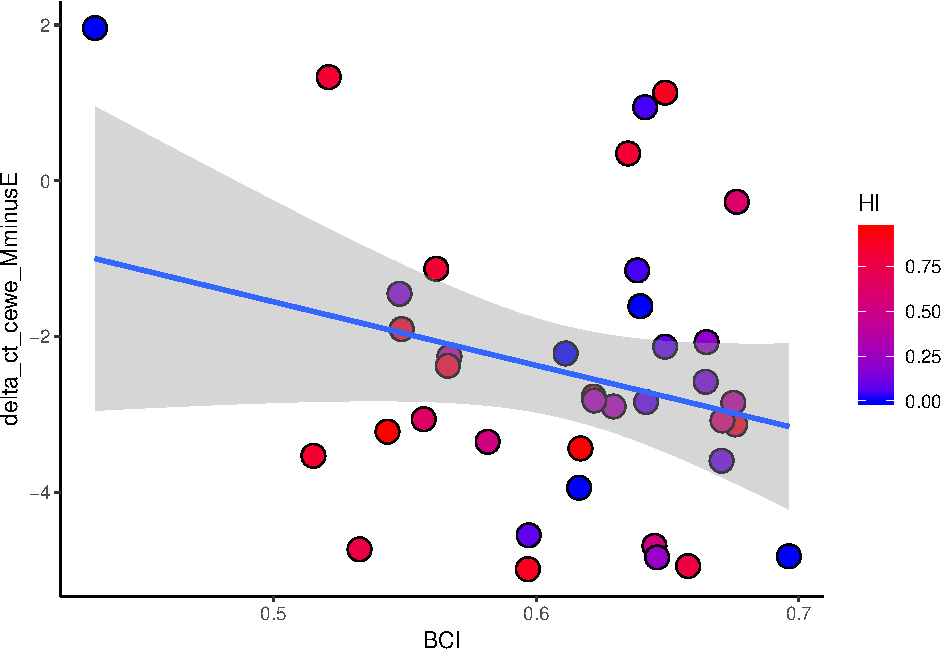
\includegraphics{Data_Analysis_Alice_files/figure-latex/unnamed-chunk-1-5.pdf}

\begin{Shaded}
\begin{Highlighting}[]
\KeywordTok{summary}\NormalTok{(}\KeywordTok{lm}\NormalTok{(ferrisiDFqpcr}\OperatorTok{$}\NormalTok{BCI }\OperatorTok{~}\StringTok{ }\NormalTok{ferrisiDFqpcr}\OperatorTok{$}\NormalTok{delta_ct_cewe_MminusE))}
\end{Highlighting}
\end{Shaded}

\begin{verbatim}
## 
## Call:
## lm(formula = ferrisiDFqpcr$BCI ~ ferrisiDFqpcr$delta_ct_cewe_MminusE)
## 
## Residuals:
##      Min       1Q   Median       3Q      Max 
## -0.14333 -0.04150  0.01148  0.04930  0.08291 
## 
## Coefficients:
##                                      Estimate Std. Error t value Pr(>|t|)
## (Intercept)                          0.591278   0.015494  38.162   <2e-16
## ferrisiDFqpcr$delta_ct_cewe_MminusE -0.008099   0.005076  -1.596    0.119
##                                        
## (Intercept)                         ***
## ferrisiDFqpcr$delta_ct_cewe_MminusE    
## ---
## Signif. codes:  0 '***' 0.001 '**' 0.01 '*' 0.05 '.' 0.1 ' ' 1
## 
## Residual standard error: 0.05654 on 36 degrees of freedom
## Multiple R-squared:  0.06604,    Adjusted R-squared:  0.0401 
## F-statistic: 2.546 on 1 and 36 DF,  p-value: 0.1193
\end{verbatim}

\begin{Shaded}
\begin{Highlighting}[]
\KeywordTok{hist}\NormalTok{(miceTable}\OperatorTok{$}\NormalTok{BCI, }\DataTypeTok{breaks =} \DecValTok{50}\NormalTok{) }
\end{Highlighting}
\end{Shaded}

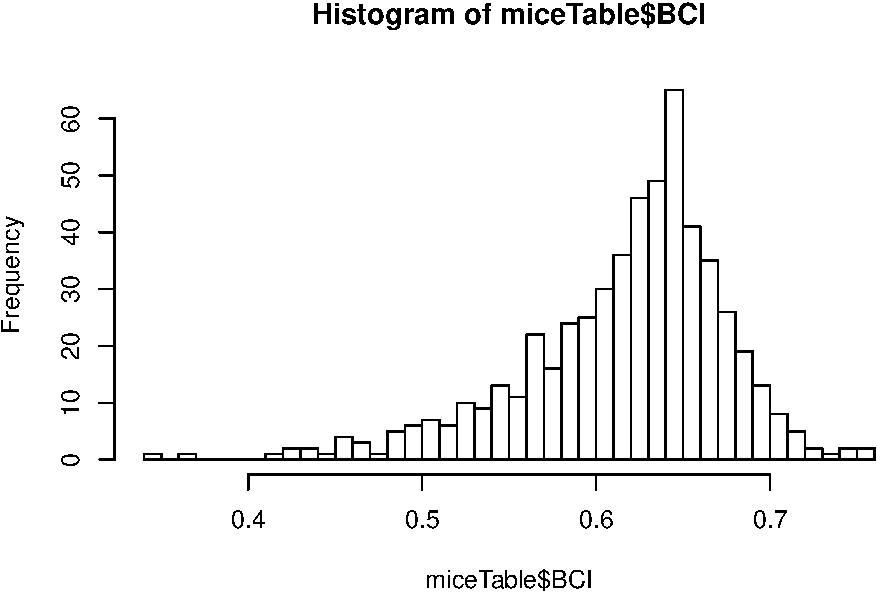
\includegraphics{Data_Analysis_Alice_files/figure-latex/unnamed-chunk-1-6.pdf}

\begin{Shaded}
\begin{Highlighting}[]
\NormalTok{## BCI vs qPCR}
\NormalTok{ferrisiDFqpcr}\OperatorTok{$}\NormalTok{delta_ct_cewe_MminusE}
\end{Highlighting}
\end{Shaded}

\begin{verbatim}
##  [1] -0.2700000 -2.1300000 -2.2166667 -2.5800000 -3.5933333 -1.1500000
##  [7] -3.9400000  0.9433333  1.9600000 -1.4500000 -2.7700000 -3.1266667
## [13] -1.9033333 -2.2533333 -4.6866667 -3.3500000 -4.8333333  1.1300000
## [19] -2.8966667 -3.0766667 -4.8200000 -2.3750000 -1.6100000 -4.5500000
## [25] -3.4350000 -4.7300000 -2.0700000 -2.8200000 -3.0600000 -4.9450000
## [31] -2.8500000 -1.1300000 -4.9850000 -3.5300000 -3.2200000  1.3300000
## [37]  0.3500000 -2.8400000
\end{verbatim}

\begin{Shaded}
\begin{Highlighting}[]
\NormalTok{ferrisiDFqpcr}\OperatorTok{$}\NormalTok{intensity <-}\StringTok{ "high"}
\NormalTok{ferrisiDFqpcr}\OperatorTok{$}\NormalTok{intensity[ferrisiDFqpcr}\OperatorTok{$}\NormalTok{delta_ct_cewe_MminusE }\OperatorTok{<}\StringTok{ }\OperatorTok{-}\DecValTok{2}\NormalTok{] <-}\StringTok{ "middle"}
\NormalTok{ferrisiDFqpcr}\OperatorTok{$}\NormalTok{intensity[ferrisiDFqpcr}\OperatorTok{$}\NormalTok{delta_ct_cewe_MminusE }\OperatorTok{<}\StringTok{ }\OperatorTok{-}\DecValTok{4}\NormalTok{] <-}\StringTok{ "low"}

\KeywordTok{ggplot}\NormalTok{(ferrisiDFqpcr, }
       \KeywordTok{aes}\NormalTok{(}\DataTypeTok{x =}\NormalTok{ HI, }\DataTypeTok{y =}\NormalTok{ BCI)) }\OperatorTok{+}
\StringTok{  }\KeywordTok{geom_point}\NormalTok{(}\KeywordTok{aes}\NormalTok{(}\DataTypeTok{fill =}\NormalTok{ delta_ct_cewe_MminusE), }\DataTypeTok{pch =} \DecValTok{21}\NormalTok{, }\DataTypeTok{size =} \DecValTok{5}\NormalTok{) }\OperatorTok{+}
\StringTok{  }\KeywordTok{facet_grid}\NormalTok{(.}\OperatorTok{~}\NormalTok{intensity) }\OperatorTok{+}
\StringTok{  }\KeywordTok{geom_smooth}\NormalTok{() }\OperatorTok{+}
\StringTok{  }\KeywordTok{theme_classic}\NormalTok{()}
\end{Highlighting}
\end{Shaded}

\begin{verbatim}
## `geom_smooth()` using method = 'loess' and formula 'y ~ x'
\end{verbatim}

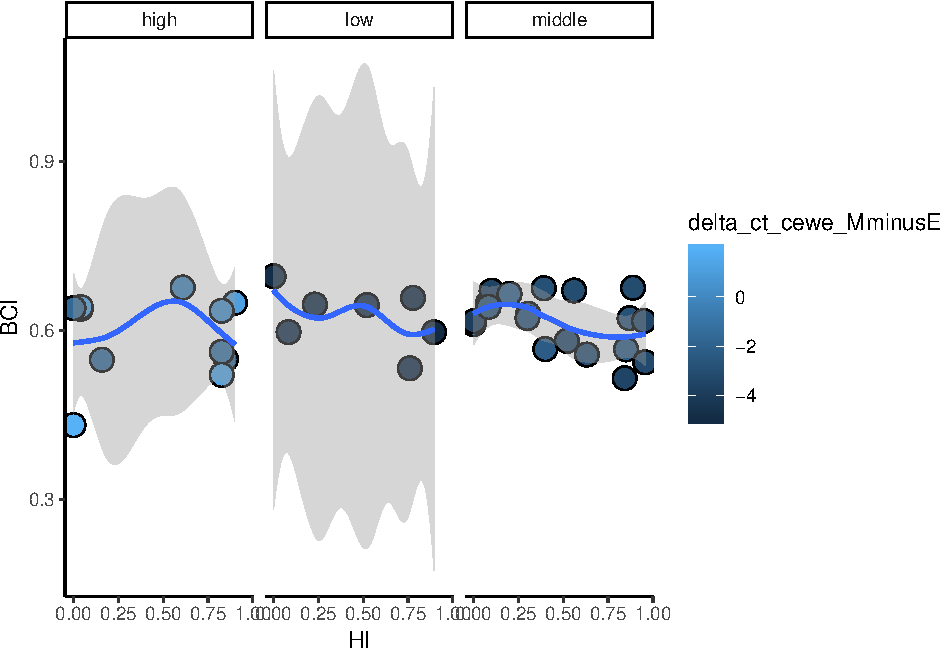
\includegraphics{Data_Analysis_Alice_files/figure-latex/unnamed-chunk-1-7.pdf}

Discussed with Stuart:

\begin{itemize}
\tightlist
\item
  Test distributions 0 or counts. Test all vs only infected
  (``intensity'') distribution. We should be able to fit the
  distribution of infected on all. Zeros are data. Stochastic move.
\item
  Separation of the zero class. balanced design case/control
  \textasciitilde{} 400 +/-70infectés SNPchip.
\item
  H0: no differences are observed
\item
  Separate \textless{}0.5 and \textgreater{}0.5 to see the species
  effect
\item
  timing : WHEN (for my thesis?)
\end{itemize}


\end{document}
